\documentclass{standalone}

\usepackage{pgfplots,mathtools}
\pgfplotsset{compat=newest}

\def\xmax{2.3}\def\ymax{1.2}

\begin{document}
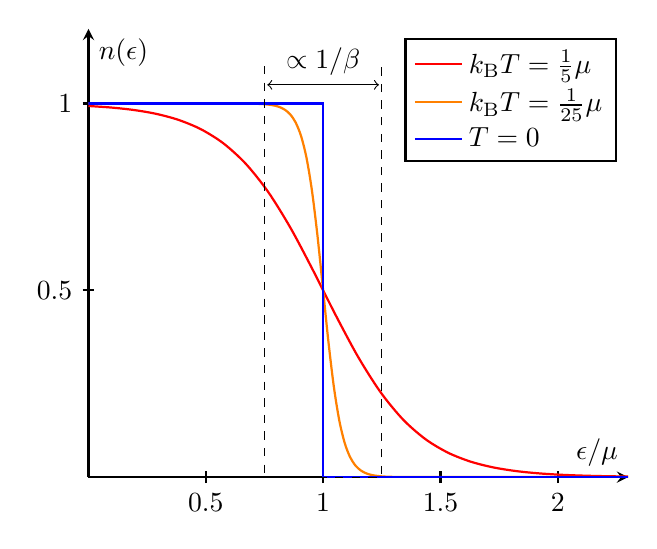
\begin{tikzpicture}
  \begin{axis}[
      xlabel=$\epsilon/\mu$,
      ylabel=$n(\epsilon)$,
      domain=0:\xmax,ymax=\ymax,
      ytick={0.5,1},
      smooth,thick,
      axis lines=center,
      every tick/.style={thick},
      legend cell align=left]

    % Graphs
    \def\chempot{1}
    \def\n#1{1/(e^(#1*(x - \chempot)) + 1)}
    \addplot[color=red]{\n{5}};
    \addplot[color=orange,samples=100]{\n{25}};
    \addplot[const plot,color=blue] coordinates {(0,1) (\chempot,0) (\xmax,0)};

    \legend{$k_\text{B} T = \frac{1}{5} \mu$,$k_\text{B} T = \frac{1}{25} \mu$,$T = 0$}

    % Thermal fluctuations
    \draw [thin,dashed] (\chempot-0.25,1.1) -- (\chempot-0.25,0) -| (\chempot+0.25,1.1);
    \draw [thin,<->,shorten >=1,shorten <=1] (\chempot-0.25,1.05) -- (\chempot+0.25,1.05) node[midway,above] {$\propto 1/\beta$};

  \end{axis}
\end{tikzpicture}
\end{document}
